\documentclass[tikz,border=8pt]{standalone}
\usepackage[T1]{fontenc}
\usepackage[scaled=0.88]{helvet}
\usepackage{amsmath,amssymb}
\usepackage{tikz}
\usetikzlibrary{arrows.meta,positioning,shapes.geometric,shapes.misc,calc,fit,backgrounds}

\begin{document}
\sffamily
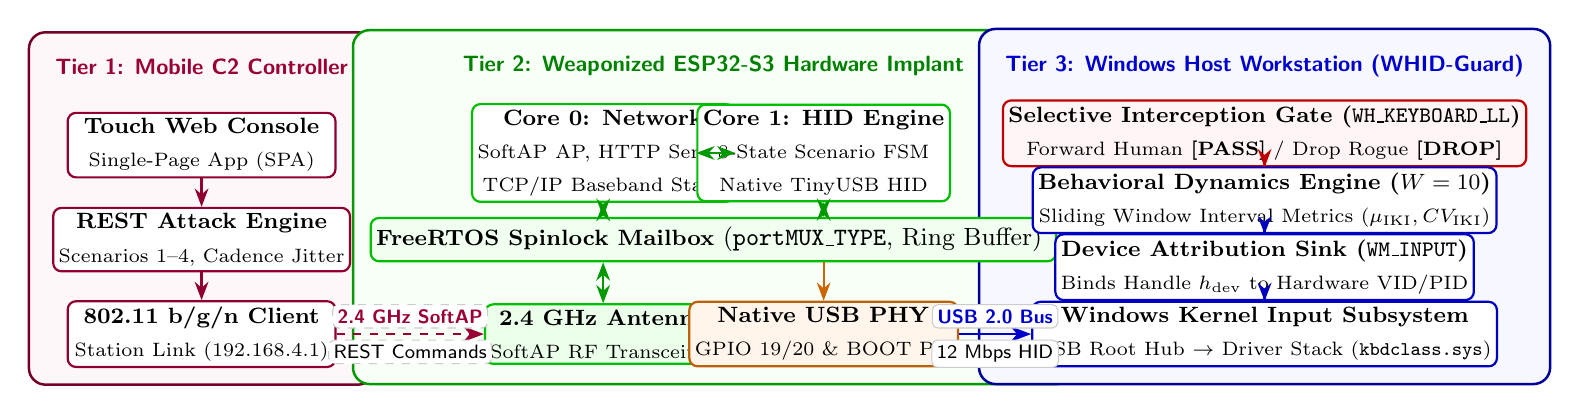
\begin{tikzpicture}[
    >=Stealth,
    font=\small,
    % Outer Container Styles
    tier_box/.style={
        rectangle,
        rounded corners=6pt,
        draw=#1!60!black,
        line width=0.9pt,
        fill=#1!3!white,
        inner sep=6pt
    },
    % Module Card Styles
    card/.style={
        rectangle,
        rounded corners=3pt,
        draw=#1!75!black,
        line width=0.8pt,
        fill=white,
        minimum width=3.4cm,
        minimum height=0.68cm,
        inner sep=2pt,
        align=center
    },
    % Badges
    badge/.style={
        font=\sffamily\scriptsize,
        fill=white,
        draw=gray!40,
        line width=0.4pt,
        rounded corners=2pt,
        inner sep=1.8pt,
        align=center
    }
]

% ==============================================================================
% TIER 1: Attack Controller (Center x = 2.0)
% ==============================================================================
\node[font=\sffamily\bfseries\footnotesize, text=purple!80!black] (t1_title) at (2.0, 2.2) {Tier 1: Mobile C2 Controller};

\node[card=purple] (c2_web) at (2.0, 1.2) {
    \textbf{\footnotesize Touch Web Console}\\[1pt]
    \scriptsize Single-Page App (SPA)
};

\node[card=purple] (c2_api) at (2.0, 0.0) {
    \textbf{\footnotesize REST Attack Engine}\\[1pt]
    \scriptsize Scenarios 1--4, Cadence Jitter
};

\node[card=purple] (c2_wifi) at (2.0, -1.2) {
    \textbf{\footnotesize 802.11 b/g/n Client}\\[1pt]
    \scriptsize Station Link ($192.168.4.1$)
};

\draw[->, line width=0.8pt, draw=purple!75!black] (c2_web) -- (c2_api);
\draw[->, line width=0.8pt, draw=purple!75!black] (c2_api) -- (c2_wifi);

\begin{scope}[on background layer]
    \node[tier_box=purple, fit=(t1_title) (c2_web) (c2_api) (c2_wifi)] (tier1_bg) {};
\end{scope}

% ==============================================================================
% TIER 2: ESP32-S3 Hardware Implant (Center x = 8.5)
% ==============================================================================
\node[font=\sffamily\bfseries\footnotesize, text=green!50!black] (t2_title) at (8.5, 2.2) {Tier 2: Weaponized ESP32-S3 Hardware Implant};

% Core 0 & Core 1
\node[card=green, minimum width=2.5cm, minimum height=0.85cm] (core0) at (7.1, 1.1) {
    \textbf{\footnotesize Core 0: Network}\\[1pt]
    \scriptsize SoftAP AP, HTTP Server\\[1pt]
    \scriptsize TCP/IP Baseband Stack
};

\node[card=green, minimum width=2.5cm, minimum height=0.85cm] (core1) at (9.9, 1.1) {
    \textbf{\footnotesize Core 1: HID Engine}\\[1pt]
    \scriptsize 8-State Scenario FSM\\[1pt]
    \scriptsize Native TinyUSB HID
};

\draw[<->, line width=0.8pt, draw=green!60!black] (core0) -- (core1);

% Mailbox
\node[card=green, fill=green!6!white, minimum width=5.3cm, minimum height=0.55cm] (ipc) at (8.5, 0.0) {
    \textbf{\footnotesize FreeRTOS Spinlock Mailbox} (\texttt{portMUX\_TYPE}, Ring Buffer)
};

\draw[<->, line width=0.8pt, draw=green!60!black] (core0.south) -- (core0.south |- ipc.north);
\draw[<->, line width=0.8pt, draw=green!60!black] (core1.south) -- (core1.south |- ipc.north);

% Hardware layer
\node[card=green, fill=green!8!white, minimum width=2.5cm] (ant_hw) at (7.1, -1.2) {
    \textbf{\footnotesize 2.4 GHz Antenna}\\[1pt]
    \scriptsize SoftAP RF Transceiver
};

\node[card=orange, fill=orange!8!white, minimum width=2.5cm] (usb_hw) at (9.9, -1.2) {
    \textbf{\footnotesize Native USB PHY}\\[1pt]
    \scriptsize GPIO 19/20 \& BOOT Pin
};

\draw[<->, line width=0.8pt, draw=green!60!black] (ant_hw.north) -- (ant_hw.north |- ipc.south);
\draw[->, line width=0.8pt, draw=orange!80!black] (ipc.south -| usb_hw.north) -- (usb_hw.north);

\begin{scope}[on background layer]
    \node[tier_box=green, fit=(t2_title) (core0) (core1) (ipc) (ant_hw) (usb_hw)] (soc_bg) {};
\end{scope}

% ==============================================================================
% TIER 3: Host Workstation (WHID-Guard) (Center x = 15.5)
% ==============================================================================
\node[font=\sffamily\bfseries\footnotesize, text=blue!80!black] (t3_title) at (15.5, 2.2) {Tier 3: Windows Host Workstation (WHID-Guard)};

\node[card=red, fill=red!4!white, minimum width=4.8cm] (host_gate) at (15.5, 1.35) {
    \textbf{\footnotesize Selective Interception Gate (\texttt{WH\_KEYBOARD\_LL})}\\[1pt]
    \scriptsize Forward Human \textbf{[PASS]} / Drop Rogue \textbf{[DROP]}
};

\node[card=blue, minimum width=4.8cm] (host_engine) at (15.5, 0.50) {
    \textbf{\footnotesize Behavioral Dynamics Engine ($W=10$)}\\[1pt]
    \scriptsize Sliding Window Interval Metrics ($\mu_{\text{IKI}}, CV_{\text{IKI}}$)
};

\node[card=blue, minimum width=4.8cm] (host_raw) at (15.5, -0.35) {
    \textbf{\footnotesize Device Attribution Sink (\texttt{WM\_INPUT})}\\[1pt]
    \scriptsize Binds Handle $h_{\text{dev}}$ to Hardware VID/PID
};

\node[card=blue, minimum width=4.8cm] (host_kernel) at (15.5, -1.2) {
    \textbf{\footnotesize Windows Kernel Input Subsystem}\\[1pt]
    \scriptsize USB Root Hub $\rightarrow$ Driver Stack (\texttt{kbdclass.sys})
};

\draw[->, line width=0.8pt, draw=blue!75!black] (host_kernel) -- (host_raw);
\draw[->, line width=0.8pt, draw=blue!75!black] (host_raw) -- (host_engine);
\draw[->, line width=0.8pt, draw=red!75!black] (host_engine) -- (host_gate);

\begin{scope}[on background layer]
    \node[tier_box=blue, fit=(t3_title) (host_gate) (host_engine) (host_raw) (host_kernel)] (tier3_bg) {};
\end{scope}

% ==============================================================================
% INTER-TIER CONNECTIONS (Clean horizontal links with spacious badges)
% ==============================================================================
% Tier 1 -> Tier 2 (Wi-Fi link)
\draw[->, line width=1.0pt, draw=purple!80!black, dashed] (c2_wifi.east) -- (ant_hw.west)
    node[pos=0.5, above=2pt, badge, text=purple!80!black] {\textbf{2.4 GHz SoftAP}}
    node[pos=0.5, below=2pt, badge] {REST Commands};

% Tier 2 -> Tier 3 (USB link)
\draw[->, line width=1.0pt, draw=blue!80!black] (usb_hw.east) -- (host_kernel.west)
    node[pos=0.5, above=2pt, badge, text=blue!80!black] {\textbf{USB 2.0 Bus}}
    node[pos=0.5, below=2pt, badge] {12 Mbps HID};

\end{tikzpicture}
\end{document}
